\documentclass{article}

\usepackage{graphicx}
\graphicspath{{figs/}}

\author{Sean Finch and Chris Pollard}
\date{2012 12 13}
\title{Nonlinear Analysis of Elementary Cellular Automata}

\begin{document}
\maketitle

\vspace{0.5in}

\begin{figure}[h!]
    \centering
    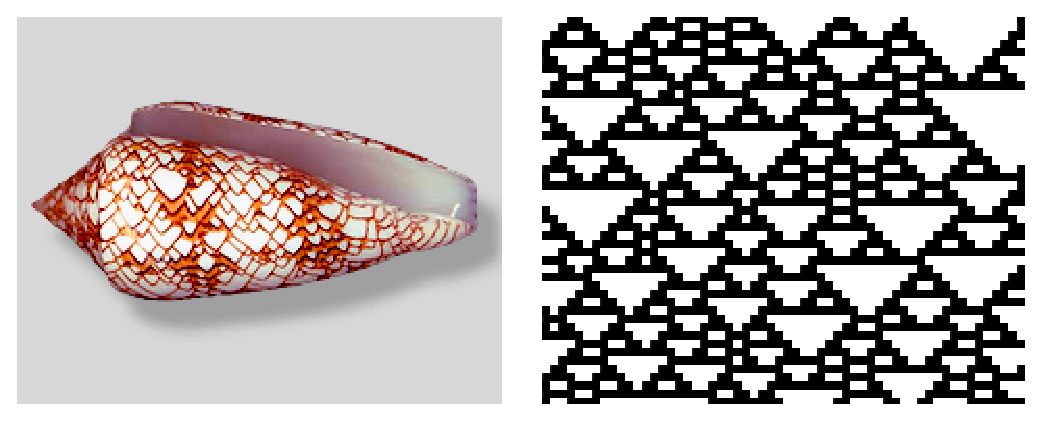
\includegraphics[width=\textwidth]{shell-automata.eps}
\end{figure}

\vspace{0.5in}

\begin{abstract}
    We present an introduction to and analysis of Elementary Cellular
    Automata (ECAs) as defined in Stephen Wolfram's
    \emph{A New Kind of Science}~\cite{anks}.
    ECAs are inherently nonlinear and their time evolution can
    exhibit extremely complex behavior--an unexpected feature given
    that their dynamics are governed by completely deterministic
    rules.
    This report demonstrates a simple analysis of several ECAs in the
    context of nonlinear systems.
\end{abstract}

\newpage

\section{Introduction}

This project is really interesting.
I think Stephen Wolfram is the smartest person ever to have stepped
foot on the earth.
When I grow up I want to work for Wolfram Research.
Cellular Automata are everywhere; just look around and you can see
them.
Even the carpeting in Bostock Library is an elementary cellular
autamaton.
Rule 122 with alternating black and white sites for initial
conditions.
See the awesome Figure~\ref{110_map}.

Something about nonlinear dynamics in general and how discrete
nonlinear systems can display complexity with a small number of
parameters--e.g. logistic map.

An Elementary Cellular Autamaton (ECA) is defined in Stephen Wolfram's
\emph{A New Kind of Science}~\cite{anks}

- Rules and rule numbering

- Examples (many figures)

\begin{figure}
\centering
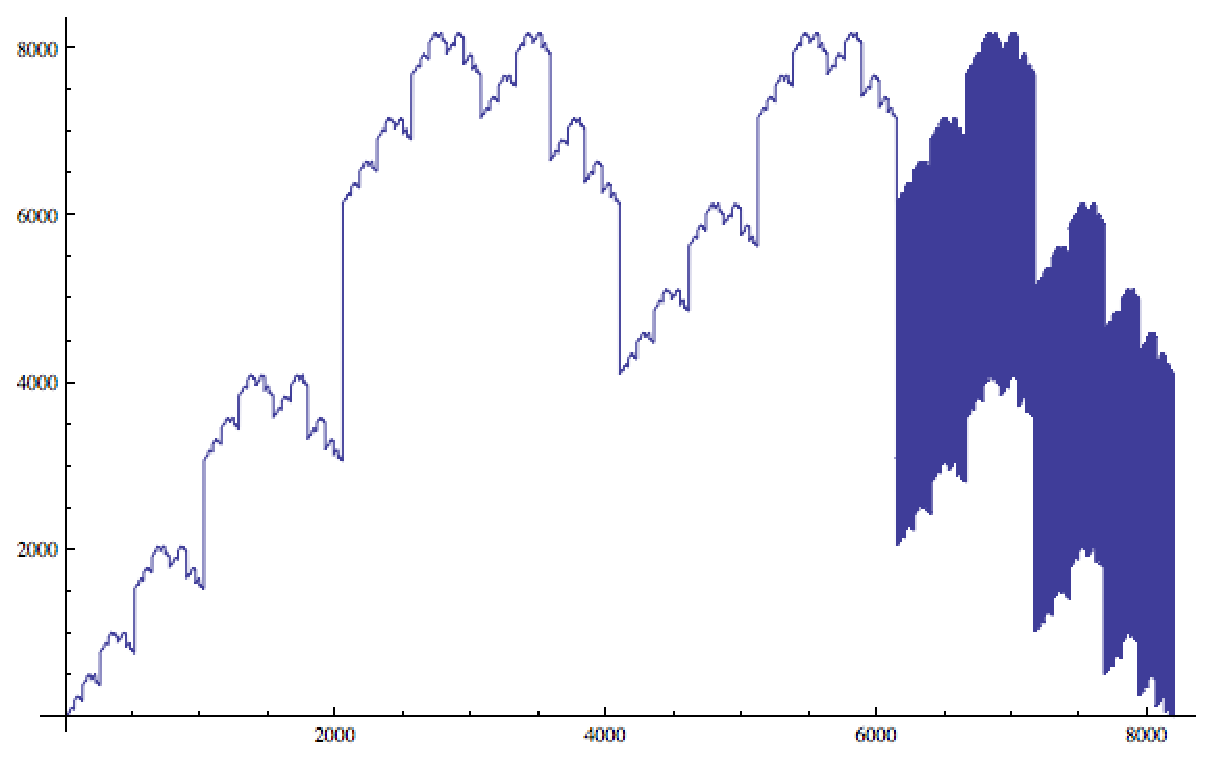
\includegraphics[width=0.49\textwidth]{110_13.eps}
\caption{\label{110_map} Fractal map for rule 110 and a 13-site grid.}
\end{figure}

\begin{figure}
 \begin{minipage}[b]{0.49\textwidth}
  \centering
  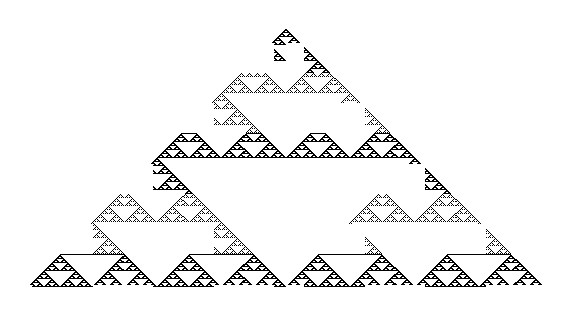
\includegraphics[width=\textwidth]{rule126.eps}
  \caption{\label{rule126} Rule 126}
 \end{minipage}
 \hspace{0.5cm}
 \begin{minipage}[b]{0.49\textwidth}
  \centering
  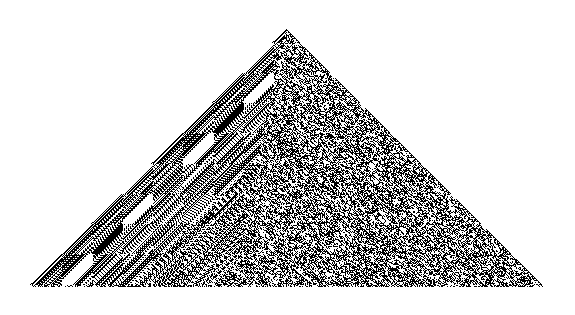
\includegraphics[width=\textwidth]{rule30.eps}
  \caption{\label{rule30} Rule 30}
 \end{minipage}
\end{figure}


\begin{figure}
 \begin{minipage}[b]{0.49\textwidth}
  \centering
  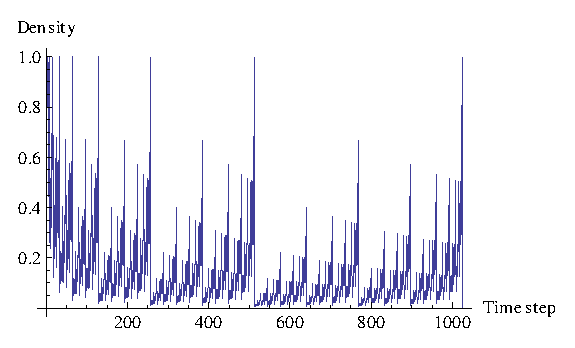
\includegraphics[width=\textwidth]{126density.eps}
  \caption{\label{126density} The Density of rule 126 plotted as a function of time step}
 \end{minipage}
 \hspace{0.5cm}
 \begin{minipage}[b]{0.49\textwidth}
  \centering
  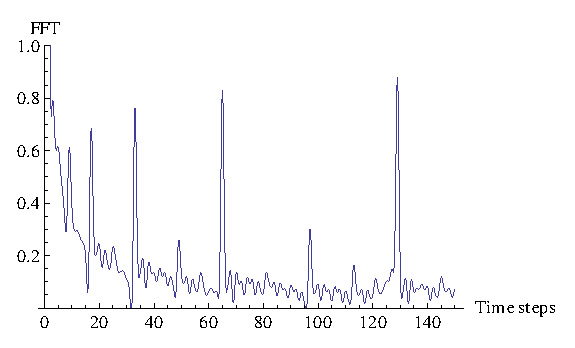
\includegraphics[width=\textwidth]{126FFT.eps}
  \caption{\label{126FFT} The FFT of rule 126's density, showing sharp peaks at 2$^n$.}
 \end{minipage}
\end{figure}


\begin{figure}
 \begin{minipage}[b]{0.49\textwidth}
  \centering
  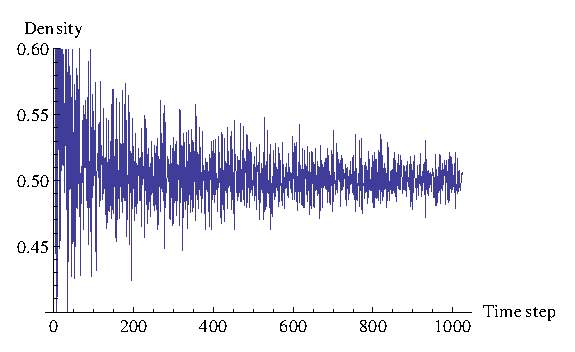
\includegraphics[width=\textwidth]{30density.eps}
  \caption{\label{30density} The Density of rule 30 plotted as a function of time step}
 \end{minipage}
 \hspace{0.5cm}
 \begin{minipage}[b]{0.49\textwidth}
  \centering
  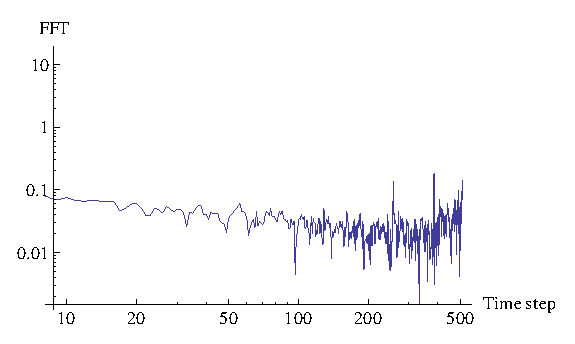
\includegraphics[width=\textwidth]{30FFT.eps}
  \caption{\label{30FFT} The FFT of rule 30's density.  The flat transform is the same as white noise.}
 \end{minipage}
\end{figure}



\section{Simple Analysis}

% TODO BETTER TITLE

An Elementary Cellular Automaton with $n$ sites per time step has
$n$ degrees of freedom.
As one studies ECAs with larger $n$ values, it becomes a daunting
task to track the state of each site at each time step, and an
analysis of the time evolution of the system as a whole becomes more
meaningful.
In order to study the general behavior of the ECA systems, we wanted
to define an observable which collapsed these $n$ degrees of freedom
into one number whose value could be traced through many time steps.
However, there are only so many such observables for such simple
systems.
One ought to choose an observable whose value is meaningful for a wide
variety of initial conditions and boundary condition constraints.


\subsection{Defining an Observable}

We chose to study on the density of black blocks as a convenient
method for collapsing the information encoded in an $n$-site ECA into
one value per time step.
For ECAs with periodic or fixed boundary conditions, the density of
black blocks is straightforward:

\begin{equation}
    \rho = \frac{n_{black}}{n},
\end{equation}

\noindent where $n$ is the number of sites in the ECA.

One must be careful in the case of ECAs without boundary conditions
because the extent of the ECA is essentially infinite, and the above
definition of the black block density is not well-defined.
However, because the ECA rules only allow the state of a block to
depend on the previous states of its immediate neighbors, by choosing
an initial condition of one black block there can be no black blocks
outside of the triangle defined by $2t+1$, where $t$ is the number of
time steps since the initial state.
Treating $2t+1$ as the effective size of the Cellular Automaton, the
density can then be redefined as

\begin{equation}
    \rho = \frac{n_{black}}{(2t+1)}.
\end{equation}


\subsection{Density Time Evolution}
% TODO MAXIMUM
For ECAs with periodic or fixed boundary conditions, there is a
maximum number of states available to the system: if there are $n$
sites and each must have a value of 0 or 1, there will be $2^n$
states.
As such, after a maximum of $2^n$ time steps the system must return to
a state that it has visited previously.

However, ECAs with no boundaries have access to an infinite number of
states.

 - FFT and Autocorrelation of density for different rules

 - Periodic Boundary Conditions

\section{Discrete Maps}

\section{Conclusion}

ECA show the remarkable property that simple, completely deterministic rules can lead to complex and chaotic behavior.  Many complex extensions to ECA exist.  An example is ECA where each cell may take on more than two values, such as tricolored CA or even allowing cells to be valued by a continuous number.  The 2D extension to ECA commonly discussed is the “game of life,” which takes place on a 2D binary valued lattice.  In this case a cell black (“living”) cell with less than two (underpopulation) or more than three (overcrowding) neighbors dies off, and white cells turn on if they have exactly three neighbors (reproduction).  The “game of life” may be thought of a simple, discrete model for processes such as bacterial growth and also exhibits interesting nonlinear phenomena.  

\subsection{Application in Cryptography}

One possible application of ECA is cryptography.  Cryptography relies on having an encrypting function that is easy to computationally compute in one direction, but inverse is extremely computationally intensive without knowledge of the key.  ECA fits this description: a binary sequence my be encrypted by applying an ECA rule and iterating over several time steps.  Determining the inverse is much harder since each cell is not uniquely determined, but depends on its also undermined neighbor.  Furthermore, the sensitivity to initial conditions implies that a one bit error in decoding the message will affect the entire message after many iterations.  To efficiently decode the message, one would use a key containing additional information, such as the ECA rule used, the format of initial conditions, and number of iterations.  The inverse of ECA then becomes solvable on a reasonable time scale.  


\appendix
\section{Code}

\begin{verbatim}

n = 1024;
m = CellularAutomaton[126, {{1}, 0}, n];
sumBlacks = Total[m, {2}]; 
Do[
  sumBlacks[[i]] = sumBlacks[[i]]/(2*(i - 1) + 1)
  , {i, 1, n + 1}
]

ArrayPlot[m, Frame->False]
ListLinePlot[Take[sumBlacks, n - 1], PlotRange -> All]
ListLinePlot[Abs[Take[Fourier[sumBlacks], 100]],  PlotRange -> {0, 1},
  InterpolationOrder -> 2]


\end{verbatim}


\bibliographystyle{plain}
\bibliography{bib}

\end{document}
